% NSF proposal generation template style file.
% based on latex stylefiles written by Stefan Llewellyn Smith and
% Sarah Gille, with contributions from other collaborators.
%
\documentclass{proposalnsf}
 
\usepackage{comment}
\usepackage{xspace}
\usepackage{graphicx}
\usepackage{subcaption}
\usepackage[hyphens]{url}
%\usepackage{cite}  - cite package clashes with natbib package used by proposalnsf.cls
\setcitestyle{numbers,comma,square}
%\usepackage[colorlinks=false]{hyperref}
% Source: https://tex.stackexchange.com/questions/823/remove-ugly-borders-around-clickable-cross-references-and-hyperlinks
\usepackage[hidelinks]{hyperref}


\usepackage{wrapfig}
\usepackage[export]{adjustbox}

\usepackage[font={small,it},labelfont=bf]{caption}

\usepackage{enumitem}
\setitemize{noitemsep,topsep=0pt,parsep=0pt,partopsep=0pt}

\usepackage{amsmath}
\DeclareMathOperator*{\argmax}{argmax}
\DeclareMathOperator*{\argmin}{argmin}

\usepackage{cleveref}   % package to refer to reference multiple labels with range option
% Using the section symbol for both \cref and \Cref commands
\crefname{section}{\S}{\S\S}
\Crefname{section}{\S}{\S\S}


\usepackage{pifont}  % for circled numbers in text refering to the figure
\usepackage{xspace}

\usepackage[table]{xcolor}
\usepackage{booktabs}
\usepackage{multirow}
\usepackage{tabularx}
\usepackage{makecell}  % awesome package that makes life so easy when making tables!
\definecolor{lightgray}{gray}{0.9}  % adjust color - used for supporting alternate table colors


\usepackage{tikz}
\usetikzlibrary{arrows.meta, positioning}


\usepackage{pgfgantt}


% Use this package for circles in text.
% https://mirror.las.iastate.edu/tex-archive/macros/latex/contrib/circledsteps/circledsteps-manual.pdf
\usepackage{circledsteps}
\pgfkeys{/csteps/inner ysep=2pt}
\pgfkeys{/csteps/inner xsep=0.5pt}
\pgfkeys{/csteps/inner color=white}
\pgfkeys{/csteps/fill color=black}

\graphicspath{{images}}


%%% Saving Space %%%
\usepackage{times}
\usepackage[subtle]{savetrees}
\usepackage[noindentafter]{titlesecfix}
\titlespacing\section{0pt}{12pt plus 4pt minus 2pt}{2pt plus 2pt minus 2pt}
\titlespacing\subsection{0pt}{12pt plus 4pt minus 2pt}{1pt plus 2pt minus 2pt}
\titlespacing\subsubsection{0pt}{12pt plus 4pt minus 2pt}{0pt plus 2pt minus 2pt}
%%% ============ %%%


\usepackage{wrapfig}


\usepackage{scalerel}


\usepackage{xcolor}
\newif\ifshowtodos
\showtodostrue  % comment this line out to hide TODOs

\newcommand{\todo}[1]{%
  \ifshowtodos
    \textcolor{red}{\textbf{[TODO: #1]}}%
  \fi
}


% See this file for a set of pre-defined journal abbreviations
\newcommand{\jas}{{\it J. Atmos. Sci.}}
\newcommand{\jpo}{{\it J. Phys. Oceanogr.}}
\newcommand{\JPO}{{\it J. Phys. Oceanogr.}}
\newcommand{\jfm}{{\it J. Fluid Mech.}}
\newcommand{\jgr}{{\it J. Geophys. Res.}}
\newcommand{\JGR}{{\it J. Geophys. Res.}}
\newcommand{\jmr}{{\it J. Mar. Res.}}
\newcommand{\arfm}{{\it Ann. Rev. Fluid Mech.}}
\newcommand{\dsr}{{\it Deep-Sea Res.}}
\newcommand{\dao}{{\it Dyn. Atmos. Oceans}}
\newcommand{\jam}{{\it Journal of Applied Meteorology}}
\newcommand{\phfl}{{\it Phys. Fluids}}
\newcommand{\phfla}{{\it Phys. Fluids A}}
\newcommand{\PhilTrans}{{\it Philosophical Transactions of the Royal Society, London}}
\newcommand{\gafd}{{\it Geophys. Astrophys. Fluid Dyn.}}
\newcommand{\gfd}{{\it Geophys. Fluid Dyn.}}
\newcommand{\PCE}{{\it Physics and Chemistry of the Earth}}
\newcommand{\PRL}{{\it Physical Review Letters}}
\newcommand{\ProgOc}{{\it Prog. Oceanography}}
\newcommand{\WHOITR}{Woods Hole Oceanographic Institution Technical Report, WHOI-}
 
\newcommand{\degrees}{$\!\!$\char23$\!$}
\renewcommand{\refname}{\centerline{References cited}}
% This handles hanging indents for publications
\def\rrr#1\\{\par
\medskip\hbox{\vbox{\parindent=2em\hsize=6.12in
\hangindent=4em\hangafter=1#1}}}
\def\baselinestretch{1}
%%%%%%

\newcommand{\phani}[1]{\textcolor{orange}{[(Phani): #1]}}
\newcommand{\BfPara}[1]{\vspace{1mm}{\noindent\bf#1.}\xspace\xspace}
\newcommand{\eg}{e.g.,\xspace}
\newcommand{\ie}{i.e.,\xspace}
\newcommand{\etc}{etc.\xspace}
\newcommand{\tsref}[1]{\textsection\ref{#1}\xspace}


\newcommand{\sysname}{{\textsc{C-frame}}\xspace}

\newcommand{\captcha}{{\textsc{captcha}}\xspace}
\newcommand{\Captcha}{{\textsc{Captcha}}\xspace}

\graphicspath{{images/}}

\usepackage{tikz}

\newcommand*\blackcircled[1]{\tikz[baseline=(char.base)]{
            \node[shape=circle, fill=black, text=white, inner sep=1pt] (char) {\footnotesize #1};}}


\DeclareRobustCommand{\bino}{%
  \begingroup\normalfont
  \includegraphics[height=1.3\fontcharht\font`\B]{binoculars.pdf}%
  \endgroup
}

% Source: https://tex.stackexchange.com/questions/139143/how-to-set-an-inline-figure-matching-the-text-height
\DeclareRobustCommand{\binoone}{%
  \begingroup\normalfont
  \includegraphics[height=1.1\fontcharht\font`\B]{bino1.pdf}%
  \endgroup
}

\DeclareRobustCommand{\binotwo}{%
  \begingroup\normalfont
  \includegraphics[height=1.1\fontcharht\font`\B]{bino2.pdf}%
  \endgroup
}

\DeclareRobustCommand{\binothree}{%
  \begingroup\normalfont
  \includegraphics[height=1.1\fontcharht\font`\B]{bino3.pdf}%
  \endgroup
}

\DeclareRobustCommand{\binofour}{%
  \begingroup\normalfont
  \includegraphics[height=1.1\fontcharht\font`\B]{bino4.pdf}%
  \endgroup
}

\DeclareRobustCommand{\binofive}{%
  \begingroup\normalfont
  \includegraphics[height=1.1\fontcharht\font`\B]{bino5.pdf}%
  \endgroup
}


\begin{document}
%\bstctlcite{bstctl:nodash}


%\renewcommand{\thepage} {B--\arabic{page}}
\pagenumbering{gobble}

\begin{center}
    {\bf CAREER: Leveraging Scambaiting Community Knowledge to Defend Against \\Interactive Social Engineering Attacks}
    %{\bf CAREER: A Data-driven Approach to Defend Against Human-in-the-loop Social Engineering Attacks}
    %{\bf CAREER: A Data-driven Pipeline for Combating Multi-Channel Tech Support Scams}  
    %{\bf CAREER: Defending Against Victim-initated Scam Telephone Calls}  
    %{\bf CAREER: A Data-driven Approach to Defend Against Human-in-the-loop Scams}
    % DHS title: A Scalable Framework for Automated Investigation of Tech Support Scams 
    \\*[1mm] Phani Vadrevu \\
    % 
     \vspace{-8pt}
\end{center}

\vspace{4pt}
\noindent
{\bf Overview}~~

Despite arguably being simple in nature to defend, there exist no tools to defend againsts them. While anti-phishing research has flourished due to plentiful access to data... samething has not happened to interactive social engineering attacks...


\vspace{4pt}
\noindent
{\bf Keywords:}~~ [TODO!] systems; information protection; digital forensics; secure software development; 


\vspace{4pt}
\noindent
{\bf Intellectual Merit}~~ 


%Our project is structured in the form of three research thrusts that assume different vantage points in the bot farm attack pipeline to help measure and mitigate bot ataks.

\BfPara{Thrust-1: Scam baiter studies}

% This includes initial qualitative research to create a first-of-its-kind taxonomic classification of in-the-wild bot attacks.
%The follow-up activity in this thrust that extends till the end of the project period is to deploy the framework and subject the data to a mixed-methods analysis that combines inital qualitative research methods for a first of its kind taxonomical categorization of in-the-wild bot attacks. This will be complemented with scalable predictive ML approaches for longitudinal insights into real world bot threat patterns. 

\BfPara{Thrust-2: Automated scam baiting}

%\BfPara{\underline{Mitigating bot farm attacks:}}
\BfPara{Thrust-3: Real-time scam call detection}


\vspace{4pt}
\noindent
{\bf Broader Impacts}~~ 
Legal/law enforcement, Older adult education, 










\newpage



% reset page numbering to 1.  This is helpful, since the text can only
% be 15 pages, and reviewers will want to believe we've kept within
% those limits

%\pagenumbering{arabic}
%\renewcommand{\thepage} {D--\arabic{page}}
\pagenumbering{gobble}

\newpage

\noindent{\Large \bf PROJECT DESCRIPTION}

\section{Research Overview}
\label{sec:overview}


Social engineering attacks on the internet can range from fully automated schemes to those involving real-time, adaptive communication by human adversaries. In this proposal, we focus on the latter, which we refer to as \textbf{Interactive Social Engineering (ISE) attacks}. These attacks involve scammers who exert sustained, interactive control over victims through multi-platform, real-time communication. Switching between communication channels is often used deliberately to avoid detection and maintain the victim's engagement. In contrast to traditional, non-interactive vectors such as phishing websites, where the static, predefined attack content is relatively easy to collect, ISE attacks rely on high degrees of human interactivity, making real-world data collection particularly challenging. This scarcity of representative datasets has, in turn, contributed to a significant gap in development of practical defenses against ISE threats. We now discuss three major representative examples to characterize these attacks.

%These scams coax victims to call fake technical support centers via various methods such as malicious advertisements, search engine poisioning, phishing emails and robocalls. Upon calling, victims who are usually targeted to be older adults are directed to share their screens under the pretext of debugging various technical support issues such as software or hardware configuration, malware mitigation. While there are many ways criminals can monetize the scam from this point, one popular method is convince the victims during these screen sharing sessions into paying for an annual support product. Unfortunatley, this is a fake-av malware that can ``freeze'' victims' operating systems on-demand and display a tech support number to initiate calls from vicitms on demand. This acts as a second entry point for a follow-up more grievous social engineering attempt by the criminals in which they transfer funds from victims' bank accounts in real-time in what is referred to as a ``Refund scam''. It is to be noted that in 2025 alone, tech-support scams account for more than a billion dollars of lost funds in the US according to the FBI's Internet Crime Complaint Center (IC3) Annual Report~\cite{}. 
\BfPara{1. Tech-support scams} Tech-support scams coax victims into calling fake technical support centers through various methods such as malicious advertisements~\cite{seacma,MiramirkhaniSN16}, search engine poisoning~\cite{SrinivasanKMANA18}, phishing emails~\cite{tasr}, and robocalls~\cite{PrasadDRR23}. Upon being persuaded to call, victims, who are typically older adults, are given real-time instructions to install remote desktop sharing software and share their screens under the pretext of debugging technical issues such as software or hardware configuration or malware mitigation. While there are many ways criminals can monetize the scam from this point, a common method involves convincing victims during the screen-sharing session to pay for an annual support product. Unfortunately, this product is actually fake antivirus malware that can ``freeze'' victims' operating systems on demand and display a tech support number to prompt further calls. This serves as a second entry point for a follow-up, more grievous social engineering attack, during which criminals manipulate victims into transferring funds from their bank accounts in real time—an attack referred to as a refund scam~\cite{tasr}.

% ABOVE ADD ANOTHER CITE TO YOUTUBE VIDEO.
This intentional transfer of funds allows criminals to bypass defenses such as multi-factor authentication, which are pervasively deployed in modern-day web applications and would otherwise require compromising an additional device such as the victim's phone. In 2024 alone, tech-support scams resulted in over \$1.4 billion in reported losses in the U.S., according to the FBI's Internet Crime Complaint Center (IC3)~\cite{ic3_report_24}. Reported losses from these scams rose by 14\% in 2023 and 58\% in 2024, underscoring the growing severity of the threat. Since many victims are unaware they have been targeted, this figure likely underrepresents the true scale of financial harm. Given the substantial economic impact of these scams and the intricate interactions they involve, we treat tech-support scams as a canonical form of ISE attacks and designate them as one of the primary focal points for defense in this project.
\todo{Add cite for how long this has been going on. I remember this being mentioned during Dubai trip (2012??)}


%Furthermore, these reported losses increased by 14\% and 58\% in 2023 and 2024 respectively, indicating the growing seriousness of this issue. Given that many victims of these attacks remain unaware of their incidence, this figure represents only a conservative estimate, highlighting the extent of financial damage potentially caused by these scams. Given the significant monetary losses caused by this scam and the complex interaction modes between scammers and victims, we consider tech-support scams a prominent example of ISE attacks and make it one of our main targets for defense in this project.


% NOTE TO ME (PHANI)
% I WANT TO CITE PROSPER PAPER BELOW -- BUT IT WEAKENS THE NARRATIVE ABOUT TOTAL COSTS OF THE ATTACKS.
% SO, I WILL SKIP THAT.
% NOTE TO ME (PHANI)
\BfPara{2. Cryptocurrency credential theft} Another upcoming example of ISE attacks is in the domain of cryptocurrencies. Recently, the PI uncovered the widespread nature of interactive scams on social media platforms, where scammers impersonate cryptocurrency exchanges~\cite{honeytweets}. These attackers exploit social media APIs on X to automate initial contact with potential victims. Subsequently, they steer victims to scammer-in-the-loop conversations on other platforms such as Instagram, Telegram or e-mail. This cross-platform handoff prevents any single platform from gaining end-to-end visibility into the scam, thereby thwarting remedial actions. Using real-time social engineering tactics, the attackers ultimately persuade victims to reveal key phrases associated with their cryptocurrency wallets. The study documented over \$1 million USD in Bitcoin stolen through these methods.
%Both US-based government agencies and cryptocurrency platforms cited similar attacks happening via telephony channel as well in which victims are directed to open their web browser and visit tailored phishing sites in their web browsers ~\cite{ic3_crypto_psa,coinbase_psa}. 
%Both U.S.-based government agencies and cryptocurrency platforms have reported similar. 
More dangerously, ISE attacks occurring via telephony channels are also reported, where scammers social engineer the victims into giving up their cryptocurrency wallet credentials~\cite{coinbase_psa,ic3_crypto_psa} leading to immediate and irreversible monetary losses. This is unlike traditional password-stealing phishing attacks where attackers still need to devise post-attack monetization strategies for the stolen data. 
%%% [CANDIDATE FOR REMOVAL] BELOW CAN BE REMOVED?
%It is worth noting that, beyond ISE-based credential theft, the cryptocurrency space is also plagued by several other fraudulent schemes such as pump-and-dump operations~\cite{XuL19}, fake giveaways~\cite{LiLG23,0001KMISTTVM24,LiYN23}  as well as adapted versions of ENS threats like domain dropcatching~\cite{MuzammilWBN24} and typosquatting~\cite{MuzammilWHKN24}. 
% and investment scams~\cite{SiuH23,SiuHV022,VasekM15},
It is worth noting that, while cryptocurrency space is plagued by a wide spectrum of social engineering attacks including fake giveaways~\cite{LiLG23,0001KMISTTVM24,LiYN23} and ENS threats~\cite{MuzammilWBN24,MuzammilWHKN24}, in this project, we focus exclusively on that rely on sustained human interaction for financial deception. In 2024, the FBI's IC3 report~\cite{ic3_report_24} attributed over \$1.1 billion in U.S. losses to cryptocurrency credential theft, highlighting the growing financial impact of ISE-based attacks.

%In the context of the current example of cryptocurrency credential break attacks, FBI's IC3~\cite{ic3_report_24} reported that it resulted in  in over \$1.1 billion USD in losses in the U.S. in 2024. This underscores the significant role that ISE-based attacks are playing in driving financial harm.

\BfPara{3. Pig butchering scams} While the previous two examples involve relatively short-lived interactions, pig butchering scams represent a long-term form of ISE attack in which the adversary builds sustained rapport with the victim over weeks or months. These scams often begin with a seemingly accidental text message, evolving into daily conversations that mix elements of romance and financial advice~\cite{xie2025did,oak2025hello,han2025anatomy}. Eventually, the victim is introduced to a web-based fake cryptocurrency investment platform that is highly tailored to them. Through fabricated returns, victims are convinced to deposit increasing amounts of money, often hundreds of thousands of dollars, into these scam platforms, typically using cryptocurrency~\cite{irs_psa_pig_butchering,xie2025did,oak2025hello}. These scams have had devastating consequences, including 42 reported suicide attempts in 2024~\cite{ic3_report_24}, as well as a widely publicized case that same year where a victim took their own life after being defrauded by a pig butchering scam~\cite{pig_butchering_suicide_report}. According to the FBI's IC3 2024 report, losses due to investment fraud reached \$5.8 billion USD, with over 58\% of victims under the age of 50, marking a striking contrast with the older demographic typically affected by tech-support scams~\cite{ic3_report_24}.

%While the above two examples mention interactions of short term effect, pig butchering scams are ISE attack examples where the interactions happen over much longer intervals of time such as months~\cite{xie2025did,oak2025hello,}. Starting as a serendepitious text message, victims' accounts show how pig butchering scams are a hybrid mixture of romance and investment scams~\cite{han2025anatomy} that ultimately introduce the victim to a highly tailored scam website that promises to be an investment platform. After showing some fraudulent investment returns, victims are ultimately scammed of hundreds of thousands of dollars via cryptocurrencies~\cite{irs_psa_pig_butchering,xie2025did,oak2025hello} resulting in reports of suicide attempts (42 in 2024~\cite{ic3_report_24}) and even tragic loss of life~\cite{pig_butchering_suicide_report}. FBI's IC3 2024 report states a lost of about \$5.8 billion USD with more than 58\% of these losses targeting population aged below 50 years unlike tech support scams~\cite{ic3_report_24}. 

\todo{CITE cross border nature of the scams overall using some exmaples like\cite{han2025anatomy}}

%It remains difficult to separate out the impact of these ISE-based attacks from many other kinds of scams plaguing the cryptocurrency realm such as giveaways via bots or streams~\cite{LiLG23,0001KMISTTVM24,LiYN23}, pump-and-dump and other investment scams~\cite{SiuH23,SiuHV022,XuL19,VasekM15}, or typosquatting fraud~\cite{MuzammilWHKN24}. However, FBI's IC3 annual report does establish the overall reported monetary loss due to  
%This multi-channel usage again makes it difficult to 

% NOTE TO ME (PHANI)
% By using multiple classes abvoe, we can go beyond the issue of this being a TSS-only project. 
% NOTE TO ME (PHANI)

%Example-1: PI's work. etc.
% I will talk about this in a bit may be, the fact that not much work exists in either of these cases?

%, if one were to get a representative dataset of fine-grained datasets such as the transcripts made by the scammers during the calls or the UI events being convinced to be made by the victims duirng the calls, it would be easy to both ``generate'' and ``evaluate'' detection solutions. Unfortuantely, most such data does not exist and we only have to rely on stories recounted by victims who are already under emotional trauma of real-world ``call scripts'' that scammers use when making these telephone calls, it might be reasoble to assume that it would be easy to generate a telephone call 

The substantial financial damages being incurred due to ISE attacks makes it clear that this remains an important and growing problem in today's society. As we discuss further in Section~\ref{sec:related_work}, most prior work has focused on detecting the precursors to ISE attacks such as malicious advertisement, scam websites and robocalls rather than building defenses aimed at directly detecting the content of the attack itself. We argue that the primary reason for the lack of such defenses is the absence of a real-world, representative ISE attack dataset -- a problem that we aim to address in this research. \todo{Add cites here}

As a contrasting example, we consider a well studied non-interactive social engineering attack:phishing emails that lead victims to password-stealing phishing websites. This non-interactive nature of this attack, solely comprising two static components, makes it feasible to collect large scale data. For instance, vigilant users who recognize the attack can ``report'' the email to security entities who leading to large-scale phishing databases (\eg OpenPhish, APWG and Phishtank). This exemplary attack data has in turn driven extensive academic research work aimed at analyzing~\cite{TianJ0Y018,PengXQ0VW19,OestZWNBZTDA20,crawlphish,SubramaniMSVP22,Sanchez-RolaBBB23,0004HK24,LimPK24,LeeLK0K25,LimLJ0KK25} and defending against~\cite{ZhangHC07,afroz2009phishzoo,AbdelnabiKF20,spartacus,LiHDLCOLH24} phishing websites. In addition, data sources such as the Certificate Transparency Logs have also stimulated defensive research enabling discovery of zero-day phishing websites in the wild~\cite{DrichelDBM21,KondrackiASN21,BijmansBSNW21,phishpedia,phishintention,dynaphish,phishllm,Teoh0LHD24}. This real-world attack knowledge has also fueled the design of more phishing-resistant user interfaces in both web browsers~\cite{EgelmanCH08,LinGTMA11,AkhaweF13,ThompsonSSWSF19,0002JW021} and email applications~\cite{Hu018,PetelkaZS19,cooper2021heads,YuAKWW23}. 


The key takeaway is that, while the wide availability of data has spurred significant research into non-interactive social engineering attacks, the same does not hold for ISE attacks. A cognizant victim typically disengages from the scammer as soon as they realize the deception. Even when a gullible victim maintains extended interaction, the exchange often spans multiple channels (\eg phone, desktop screen sharing) and is rarely recorded in a format suitable for reporting. As such, unlike web-based phishing where reporting is widely supported across both organizational systems and end-user products~\cite{LainKC22,KerstenBAZ22,pilavakis2023didn,MarinBZA23,doubly_dangerous}, we are not aware of any widely deployed systems that facilitate recording and reporting of ISE attack data for further analysis. Any after-the-fact reports submitted to law enforcement agencies are limited to the victims' recollections, who are often coping with the emotional distress of being targeted. These reports suffer from limited granularity and memory-related inaccuracies, making them insufficient for driving robust detection or analysis efforts.


In the absence of deliberate and systematic defense mechanisms against ISE attacks, an unlikely group has stepped in to fill the gap: independent internet vigilantes. These individuals have taken it upon themselves to engage directly with scammers, often manually baiting them in real time to waste their time or, in some cases, to expose their operations. As this is an extremely labor-intensive process, their efforts can disrupt scams only to a limited extent. However, many of these scam baiters possess deep, experience-driven knowledge of attacker behaviors and tactics. Their work offers valuable glimpses into attacker workflows, yet the insights they generate remain scattered across isolated online spaces such as forums and Discord servers where these communities coordinate their activities. Currently, this raw and unstructured knowledge remains siloed and is not being leveraged for broader defense or educational purposes. This raises a compelling question that we aim to address in this research project: \emph{Can we systematically collect, curate, and analyze the work and expertise of these underutilized scambaiting communities to build effective defenses and educational interventions against ISE attacks?}

We attempt to address this challenge with a 4-phase research project design that will be powered by the knowledge we expect to gain from online scambaiting communities. We provide an overview of this below.

%\BfPara{Thrust-1: Scambaiting community studies} In this first thrust, we plan to conduct various kinds of user studies involving scambaiting community members. Using the knowledge from this, we plan to establish a basic taxonomy of ISE attacks targeted by the scambaiting community along with their operational characteristics. Further, we expect to gain information about the procedure used by the community members about finding new ISE attacks, the hardware and software setup used by them for interactions, and their end goals for each kind of ISE attack. We are also interested in finding information about the follow-up actions taken by the scambaiter community such as the entities to whom they report this. As scambaiting might often stretch into the offensive side, we are also interested in finding more information about what actions scammers might pursue in this regard and for what objectives. We plan to utilize interview studies that help in providing wide range of data regarding the ISE attacks that baiters have experience with historically. To complement for memory issues and missing fine-grained studies, we also plan to utilize a carefully designed, IRB-approved protocol for performing a controlled observational study of live scam baiting activities by scammers. Finally, we plan to cap off these user studies with a co-design workshop where we include the baiters in designing a blueprint for a scambaiting tool to counteract various ISE attacks. We plan to supplement these in-person studies with thematic analysis of passive communication data between scambaiting participants on various software platforms that they use for communication. This data allows us access to much finer-grained information then can be gathered from limited time human studies. We will follow up this study with both a theoretical and empirical analysis of how the techniques used by the scambaiting community relate to what is known about ISE attacks from academic research. We expect this analysis to be mutually benefical to both the scambaiting communities as well as academic researchers helping close the bridge between these two groups and letting them adapt to what is better. 


\BfPara{Thrust-1: Scambaiting Community Studies}
In the first thrust of this project, we aim to study the scambaiting community through a combination of user research methods and passive data analysis. Our goal is to understand how these volunteer actors engage with and counteract ISE attacks, and how their strategies can inform broader defense efforts. To support this work, we have already received a letter of collaboration from the founder of a popular scambaiting forum with over 25,000 registered members and more than 300 weekly active participants. We plan to recruit participants from multiple such forums and then conduct interview-based user studies with experienced members of these communities. Through these interviews, we aim to construct a taxonomy of the types of ISE attacks targeted by the community members, along with associated attacker behaviors and operational characteristics. These studies will also surface insights into how scambaiters discover new scams, the hardware and software configurations they use for engaging with scammers, and their intended outcomes across different scam scenarios. 

\begin{wrapfigure}{R}{0.65\textwidth}
  \centering
  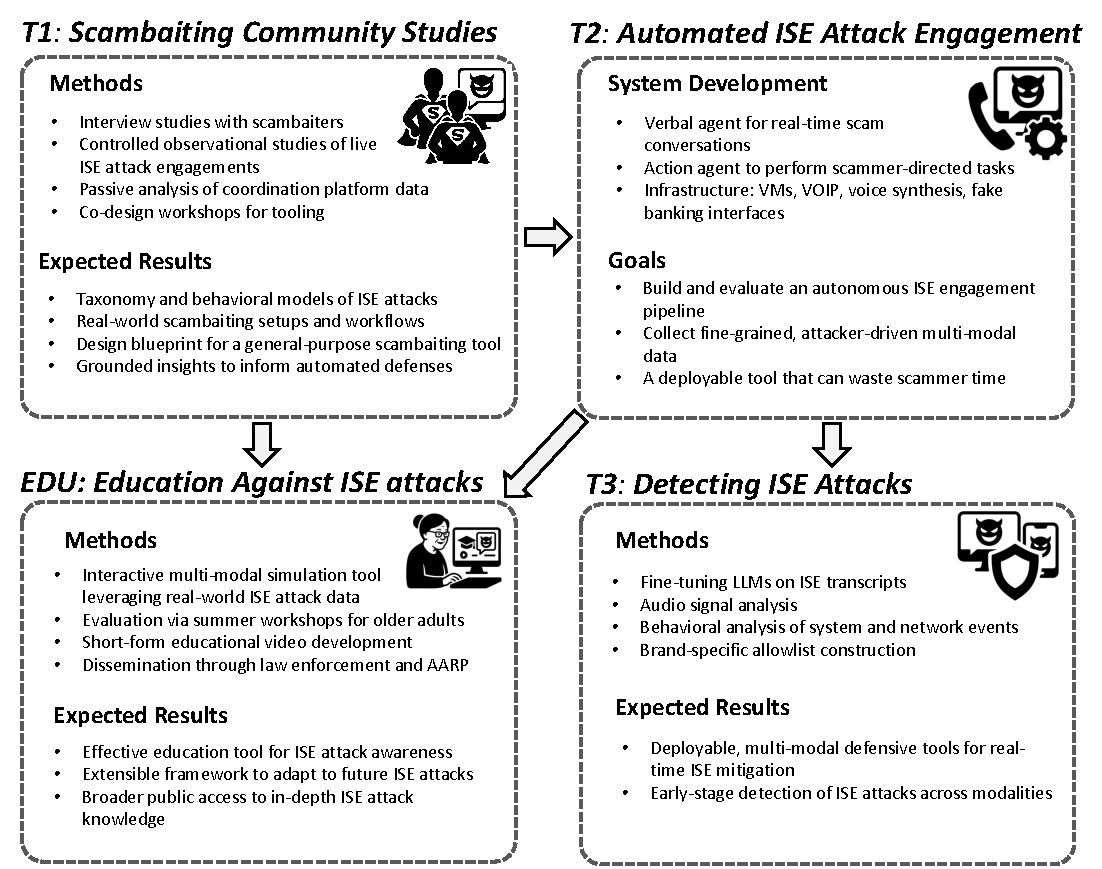
\includegraphics[width=0.63\textwidth]{images/project_overview.pdf}
  \caption{Overview of the project showing the four core thrusts: T1 (Scambaiting community studies), T2 (Automated ISE attack engagement), T3 (Detecting ISE attacks), and EDU (Education against ISE attacks). \todo{Include BI in the figure!}}
  \label{fig:project_overview}
\end{wrapfigure}
To account for recall limitations and gain more granular insights, we will complement interviews with a controlled, IRB-approved observational study of live scam baiting sessions. Additionally, we will analyze passive communication data from platforms where scambaiting communities coordinate (\eg forums, Discord). This data will provide broader and finer-grained coverage of scambaiting practices, helping to contextualize our human studies and uncover behavioral norms, technical tips, and reporting pathways. As part of the final stage in this thrust, we will conduct a co-design workshop with community members to collaboratively develop a blueprint for a general-purpose scambaiting tool. Finally, we will carry out a comparative analysis to map the techniques used by scambaiters against the academic understanding of ISE attacks. This two-way analysis will help bridge gaps between community practice and scholarly knowledge, offering mutual benefits: better-aligned defenses for the scambaiting community and more field-informed threat models for researchers.

%Our research explores how to extract, structure, and operationalize this crowdsourced knowledge to improve the broader ecosystem's resilience to ISE attacks. This research aims to bridge that gap by extracting actionable intelligence from these scattered sources and transforming it into structured datasets, threat models, and public awareness resources.

\BfPara{Thrust-2: Automated ISE Attack Engagement}
Building on insights from the scambaiting community and the observational data collected in Thrust-1, this thrust aims to design, develop, and deploy an automated pipeline capable of engaging with scammers in the wild. The system will pursue autonomous, multi-modal interactions that continue through the various stages of an ISE attack until reaching monetization. The architecture will consist of two main components: a verbal agent responsible for real-time conversation with the scammer, and an action agent that executes suggested behaviors such as enabling remote desktop access or navigating to banking websites. The system will be engineered using hardware and software components identified as practically useful by the scambaiting community. We anticipate this will include VOIP gateways, virtual machines, voice synthesizers, and replicas of financial apps and websites. Recorded calls and interaction traces from the observational studies in Thrust-1 will serve as a foundational dataset for designing, training, and evaluating this automated pipeline.

To bootstrap deployment, we will leverage both prior academic work, including the PI's research on mining ISE attack entry points in the wild~\cite{seacma,tasr,MiramirkhaniSN16,SrinivasanKMANA18,honeytweets}, and operational knowledge obtained from the scambaiting community. The system will serve dual purposes: (1) collecting fine-grained forensic and operational data about real-world ISE attack strategies, and (2) wasting scammers' time, thus acting as a direct defensive mechanism. The resulting system will generate the first large-scale dataset of attacker-driven, real-world, multi-modal ISE interactions. We are committed to upholding strong ethical standards in this thrust. One version of our study protocol, which involves live deception experiments without post-study debriefing or consent, has already been reviewed and approved by a 12-member IRB panel at our institution following extensive discussion of the legal, social, and criminological dimensions of the research.

 
\BfPara{Thrust-3: Detecting ISE Attacks}

Building on the collected real-world ISE attack datasets, this thrust focuses on developing and evaluating real-time defenses across multiple modalities, including telephony and desktop environments. These defenses will draw from the transcripts, audio content, and system-level interaction traces observed during scam engagements.

First, we will leverage parameter-efficient fine-tuning (PEFT) methods~\cite{HuSWALWWC22,DettmersPHZ23,XuXG0CZC0024} to adapt open-source large language models (LLMs) to the unique linguistic and interactional features of ISE attack transcripts derived from Thrust-2. This will enable a lightweight and practical detection pipeline capable of flagging ongoing ISE attacks as they unfold over telephony channels. A key focus will be on detecting attacks as early as possible~\cite{LiuW18,HartvigsenSKR19,RingelCFER24}, since waiting until the call progresses to a ``device compromise'' state is too late to prevent harm.

In addition to semantic signals from conversation transcripts, we will also analyze acoustic features of the audio stream. This includes both speech characteristics and background noise artifacts, which prior work has shown to be useful for mitigating malicious uses of the telephony channel~\cite{BalasubramaniyanPAHT10,KotropoulosS14,PrasadBMR20,KritsiolisK24}. Third, we will also explore detection strategies based on observed system behavior on the victims' devices. Specifically, we will study the sequence of user interface events (\eg mouse clicks, application launches) and on the victims' device and the resulting network activity that occurs either under the scammers' direction or through direct remote access.

Together, these linguistic, acoustic, and behavioral detection approaches form the foundation for a deployable defense pipeline capable of proactively identifying and interrupting ISE attacks in real time. Finally, we will construct brand-specific ISE attack allowlists by mining official contact information for commonly targeted brands identified in our earlier thrusts. These allowlists can be deployed directly by telephony carriers or endpoint devices for real-time validation and also enhance the performance of semantic detection models by serving as a reference list, following approaches used in recent work on web-based credential phishing~\cite{LiHDLCOLH24,phishintention,AbdelnabiKF20}.



% Notes: Apart from ~\cite{GuptaGBD20,BilskiJ23,RingelCFER24}, Use this link as inspiration if need be to have a "time decay factor": https://medium.com/@aditya00kumar/ranking-the-results-of-ml-models-with-a-time-decay-factor-for-large-scale-anomaly-detection-1dcf44dcd824

\BfPara{EDU: Education against ISE Attacks}
Existing educational resources for ISE attacks are typically limited to static, generic warnings that lack specificity, interactivity, and grounding in real-world scam tactics. To address this gap, we propose to develop a multimodal, interactive ISE attack simulation tool that enables users to experience realistic scam scenarios based on actual transcripts and behavioral traces collected in Thrust-2.

The tool will support branching narratives, annotations, and context-aware interactions to expose users to the multi-channel, human-in-the-loop nature of ISE attacks. We plan to design it as an extensible framework powered by generative AI, allowing us to vary instructional content and simulate diverse attack styles. We will evaluate the effectiveness of the tool through user studies conducted as part of summer workshops, with a particular focus on older adults who are especially vulnerable to these scams.

This platform will also serve as a source for generating short-form educational video walkthroughs of representative ISE attack flows. To broaden the reach of these materials, we will work with our law enforcement partners at the United States Secret Service and the local Sheriff's department to disseminate the developed videos through their community outreach and public education channels.

%a result, any after-the-fact reports submitted to agencies like the law enforcement are limited to victims' recollections, which are often insufficient for driving detection or analysis efforts due to limited granularity and memory-related inaccuracies. 


%Over the years, researchers including the PI have shown the potential for these phishing websites to also exhibit a bit of dynamicity in their content for evasive purposes which has also been studied in dept
%While we discuss a range of existing mitigatory solutions and how they fall short of combating present-day ISE attacks such as the above in Section~\ref{sec:related_work}, the financial damages being inflicted by them make it directly clear that there is a dearth of deployed solutions that neutralize their threat. Conceptually, this might be a simple problem to defend against. If one were to get a representative dataset of variuos events taking during the interactions of ISE attacks, then appropriate defensive solutions can potentially be devised based on being able to track them. 

% NOTE (TO ME): BELOW IS UNECESSARY - makes things look too simple for Thrust-3 and adds not much value.
%For example, having real-world scripts of various stories that scammers devise to direct a router configuration error into a malware issue on a user's computer that requires remote diagnosis~\cite{tasr} would be incredibly useful to devise a detection solution. Similarly, the series of specific actions performed by a victim on their computers, upon directions of the attacker (\eg opening event logger~\cite{MiramirkhaniSN16}) can also be very helpful to identify an ongoing attack. Yet, there is not much data containing real-world attacker communication so far. Unfortunately, this affects both devising as well as evaluation of any scam detection technologies. 

% NOTE-TO-SELF: IT IS BETTER TO GET RID OF THE BELOW CITATION THAN A NON-SIGNIFICANT PAPER JUST TO CONVOLUTE YOUR NARRATIVE LOGIC. KEEP IT STRAIGHTFORWARD AND TO THE POINT. 
%Instead, the limited amount of existing ISE attack defenses have relied on scripts that are artificially written by role-playing attackers~\cite{DerakhshanHB21} which does not work well given that it is driven by the scammers. 


%This project focuses on designing principled, data-driven methodologies to characterize and mitigate \emph{human-in-the-loop} social engineering attacks. In these attacks, the adversary maintains interactive control over the victims via real-time, adaptive communication them during the attack lifecycle. This can is often done via multiple platforms on multiple channels between which the attacker switches frequently as part of their strategy. We refer to these as interactive social engineering attacks (\bf{ISE}) throughout this proposal. Unlike traditional, non-interactive social engineering vectors such as phishing websites where the attack content is predefined and easy to collect, ISE attacks interactive requirements made attack data examples scarce in existence. This unfortunately led to a dearth in practical defenses for ISE attacks. 

%This project focuses on developing methodologies to study and thwart online, \emph{human-in-the-loop} social engineering attacks. Specifically, we plan to develop a multi-stage pipeline for defending against various social engineering attacks that involve interactive participation of attackers with the victims during the attack. This is in sharp contrast to non-interactive social engineering attacks such as credential phishing attacks or robocalls all of which have received significant attention from researchers until now.  ith traditional well-studied social engineering attacks such as credential phishing attacks where in the attacker only sets up a phishing website and disseminates this to the victims en masse 





-----------------------------------------------
FLOW OF THIS SECTION:

\begin{enumerate}
%\item 1. Introduce "human-in-the-loop" social engineering attacks; THe presence of "humans" makes this pretty complicated/twisty. For example, a text message from a cryptocurrency scammer will steer user to make a phone call who will then direct the user to open their computer and follow directions from there. In our recent work on crypto currency scams, we have shown the same where victims are moved from X to other platforms such as email or instagram providing additional benefits of not letting any single platform get a full-on view of the entire scam. 
%from a cryptocurrency scammer, can make the user visit

%\item 2. we present TSS scams as a representative example of this.  Owing to its complicated working nature, this will be our main focus. Money - talk about how much this alone is worth.

%\item 3. Crypto currencies are another representative example (https://www.ic3.gov/PSA/2024/PSA240801 https://www.coinbase.com/blog/hang-up-the-phone-stop-social-engineering-scams). Again money - how much is this worth overall. 

%\textbf{Note to self}: By using multiple classes, we can go beyond the issue of this being a TSS-only project. 

%\item 4. Looking back at both, if one were to get a representative dataset of fine-grained datasets such as the transcripts made by the scammers during the calls or the UI events being convinced to be made by the victims duirng the calls, it would be easy to both ``generate'' and ``evaluate'' detection solutions. Unfortuantely, most such data does not exist and we only have to rely on stories recounted by victims who are already under emotional trauma of real-world ``call scripts'' that scammers use when making these telephone calls, it might be reasoble to assume that it would be easy to generate a telephone call 

% PHANI (NOTES): MOVED THE BELOW TO T1; ITS BETTER TO SPRINKLE SOME ARGUMENTS THROUGHOUT THE PROPOSAL.
%\item 5. REGARDING SE, pretty much most of the work is on phishing in web - both measurements as well as user studies, defense etc. There's a strong reason for this. THEY HAVE LOTS OF DATA WE DON'T AND THIS MAKES IT DIFFICULT TO PURSUE DEFNESIVE MEASURES. More deeply here: In web-based credential phishing attacks, there exist a steady influx of SE attacks that are blanket-sent to everyone. Thus, they end up getting populated in blocklists. Same is not the case for human-in-the-loop attacks due to the hindrances involved in being able to gather data. natural evasive factors that disable this. As a result, most research is only using artificially generated data.   Discuss psychological factors (MOVED TO THRUST-1). 

%\item 6. Forward cite to our discussion on robocall research thus far and how it is also mainly non human-in-the-loop data driven. Better not waste too much time here as we want to talk about the main idea soon (also related work needs to have some interesting stuff too!)

%\item 7. BIG IDEA: IN THE ABSENCE OF ANY deliberate DEFENSE MECHANSISMS, a group of internet vigilantes are taking care of all this right now.  Knowledge is simply sitting in this island of isolated netowrk right now. Can we leverage this knowledge from these communities and use it to power our own defenses and educational actions? and then use it for a other boundaries? That is the main question we are trying to deal with here...

%We want to leverage them to start a 4-part pipeline for this research.


\item 8. Figure showing 4 parts (3 thrusts, 1 education)

\item 9. Thrust-1 discussion
\item 10. Thrust-2 discussion. CALLOUT ABOUT ETHICS/IRB APPROVAL ETC.
\item 11. Thrust-3 discussion.
\item 12. Edu discussion. 

\item 13. PI's past research trajectory is all devoted to realizing this big idea. In the past, focused on developing platforms for recording social engineering attacks including browser-based modification. This followed by works that used these to study web-based social engineering attacks on a large scale. These led to discovery of ecosystems involving complicated multi-channel human-in-the-loop scams with virtually no defenses other than internet vigilantes. 

\item 14. CALLOUT: THIS PI's LONG-TERM RESEARCH AGENDA IS TO WORK AGAINST THE ADAGE of "HUMAN IS THE WEAKEST LINK IN CYBERSECURITY" by developing data-driven technologies that reduce the risk as of people falling for social engineering attacks. 
REVISED (CG - ChatGPT): This PI's long-term research agenda is to challenge the prevailing adage that "humans are the weakest link in cybersecurity" by developing data-driven technologies that reduce the risk of individuals falling victim to social engineering attacks. In the context of ISE attacks, these could often be dismissed as older adults or those who are tecnologically inept to only be affected by these scams. Such a thinking is dangerous as technology should adapt to the consumers' needs and it is important to study the exact methods in which technology is being victimized.


\end{enumerate}




% -----------------------------------------------
% RANDOM NOTES FOR THIS SECTION:


% NOTES IN GENERAL:
% (1) Definitely not just TSS; baiters said they do PCH scams as well.
% (2) Perhaps, our crypto-TSS scams from SP24, or hybrid crypto-TSS (that I experienced) and ultimately, pig butchering scams all also fall under this category. 


% -----------------------------------------------

%This project focuses on developing methodologies to study and thwart victim-initiated telephony scam calls. In these scams, attackers use baits such as fake invoices or fake malware infections to ``scare'' victims into making outgoing telephone calls to the attackers. These baits are typically distributed to potential victims by abusing web search engines, online advertising networks, or email services. As only the interested victims who are already convinced by the bait make the calls, these result in ``high-quality'' opportunities for cybercriminals who then employ specialized social engineering techniques to cause real-time financial damage to them. Technical support scams, in which the attackers pretend to operate a real tech support center are a particularly problematic example of these victim-initated telephony scams. According to the FBI’s Internet Crime Complaint Center (IC3) Annual Report, U.S. victims lost over \$924 million to tech support scams in 2023 alone, with the elderly being the primary targets ~\cite{}



WHILE IN OTHER CASES, CONTEXTUAL DATA SUCH AS THE PHISHING WEBSITE, or PHISHING EMAIL or SMS can be forwarded and data can be stored, telephony conversational data is highly private - and hence detection models cannot be easily created. 



----------------
Telephony channel-based tech support scams (TSS) have become a significant societal threat, particularly targeting vulnerable populations. In these scams, cybercriminals abuse web search engines and online advertising networks to promote scam websites and persuade victims to make telephone calls to fake support centers. Figures 1 and 2 show two real world examples of TSS websites in the wild. Upon receiving calls via the phone numbers in these sites, scammers will fabricate a non-existent problem with the victims’ devices (personal computers and mobile devices), remotely connect to them, and ultimately, steal thousands of dollars as covered in many U.S. news reports [1, 2, 3]. The funds are stolen by social engineering the victims to willingly transfer the money which neutralizes any two-factor authentication (2FA) defenses that are commonly used.

According to the FBI’s Internet Crime Complaint Center (IC3) Annual Report, U.S. victims lost over \$924 million to tech support scams in 2023 alone, with the elderly being the primary targets ~\cite{}. Given that many victims of these attacks remain unaware of their incidence, this figure represents only a conservative estimate, highlighting the extent of financial damage potentially caused by these scams. Prior research, including work conducted by PI Vadrevu, has shown that this crime involves many malicious call centers operating in South Asia~\cite{}. While these call centers operate from outside the U.S., the criminals also rely on domestic money laundering networks to facilitate the illicit transfer of funds from the victims ~\cite{}. This highlights the transnational and complex nature of this crime, making it difficult to address without specialized investigative measures.

This project proposes developing multiple technologies that law enforcement agencies can utilize at scale for collecting incriminating evidence against criminals involved in tech support scam operational pipeline to aid in prosecution and mitigation efforts. As proof-of-concept, we will also deploy these technologies throughout the project period and share resulting forensic datasets with law enforcement authorities. This forms the first collection of a comprehensive tech support scam dataset with implicating information about all parties actively or passively involved in the scam pipeline. As such, this project directly aligns with Objective 4.4 to “Combat Cybercrime” in the DHS Strategic Plan for 2023-27~\cite{}. This objective is part of the department’s broader mission to secure the U.S. cyberspace. Specifically, this objective in the devised strategic plan calls for leveraging state-of-the-art cyber investigative approaches to combat cross-jurisdictional financial fraud, which is the central goal of this proposal. All the proposed tasks directly result in reusable tools, actionable insights and valuable datasets that law enforcement agencies can adopt to combat rampant tech support scams and safeguard U.S. residents.


PLAN:

Inbound telephony scams -> too much low percentage -> robocalls -> many defenses relying on data from honeypots, as well as authentication techniques. Governmental regulations also help.

Outbound telephony scams, are for some reason left out of these and are much more challenging to detect. Initiated by websites - but PI's research shows that they are not good. 

UNITL NOW NO DATA AT ALL. LITTLE WE CAN FIND IS ALL FABRICATED DATA. 


This SOK paper presents some interesting ``challenges'' that we can adapt here~\cite{TuDZA16}.


\begin{enumerate}

\item Other solutions such as STIR/SHAKN protocols mitigate the threat of inbound phone scams. [Explain how]. 
\item Works so far have also predominantly focused on reducing the threat of inbound phone scams (such as robocalls) - this is because it is more percievable.
\end{enumerate}
%\input{bg_prelim}
\section{Prior Related Work}
\label{sec:related_work}


Flow:

\begin{enumerate}
\item Overview of scam measurement/detection works done so far. 
\end{enumerate}
Matt's work on Email scam baiting~\cite{ChenWE23}. They cited this position paper as an approach for why an ``active defense'' approach is necessary~\cite{CanhamT22}.
Should this be a cite: ~\cite{BajajE23}



Some this might have to be moved to Intro section.


%LET'S HAVE A FIGURE THAT CONVEYS THIS POINT ABOUT HOW TSS SCAMS WORK PICTORIALLY AND HOW EACH SOLUTION TACKLES ONE PART OF THE PROBLEM WITHOUT ADDRESSING THE CORE!!!! THIS IS GOING TO BE A COMPLICATED FIGURE BUT UBER-COOL. 

% THE FIGURE NEEDS TO SHOW THE TARGET SPACE THAT WE ARE ULTIMATELY AIMING TO MAKE AN IMPACT AT (WITH THRUST-3). BUT, THIS HASN'T BEEN REALIZED YET. THE LIMITED ONES THAT ATTEMPT TO DO THIS ARE BASED ON SYNTHETIC DATA WHICH ALSO CANNOT BE EVALUATED DUE TO LACK OF REALWORD DATA:
THESE ARE THE LIMITED AND ONLY ISE ATTACK DETECTION WORKS THAT I KNOW OF SO FAR:
~\cite{DerakhshanHB21,}
~\cite{Zhao0LY018}

~\cite{ocleicniks2025real} LLM-based scam call detection, similar to the CHI 25 EA paper. However, only 15 fraud calls sourced from YouTube videos. Eval metrics are not good (more one shot kind)

% REBUTTAL 1.0 (NEXT DAY, LOL): MAY BE NOT? AT LEAST NOT IN INTRO. THE READER COMES WITH AN EXPECTATION THAT THE FIRST FIGURE THEY SEE IS A REPRESENTATION OF WHAT THE PI IS GONNA DO. INSTEAD, THEY END UP WITH A FIGURE ABOUT WHAT HAS ALREADY BEEN DONE. WHILE IT MIGHT CONVEY THAT THE PI KNOWS WHAT THEY ARE TALKING ABOUT, I THINK THIS IS THE WRONG PLACE TO SHOW OFF THIS THING. THIS DISTRACTS THEM FROM THE MAIN POINT. FURTHER, WHAT IS THE USE OF GIVING TWO EXAMPLES? IF THE FIGURE WILL KEEP BEATING UP ON ON EXAMPLE. IF NECESSARY, THIS "SHOW OFF" CAN BE DONE IN RELATED WORK SECTION. BUT, EVEN THAT HAS TO BE CONSIDERED CAREFULLY AS THIS IS A WASTAGE OF CRUCIAL SPACE. WE'LL SEE BUT DEFINITELY NOT HERE.

In absence of data to detect ISE attacks in channel, existing academic work has instead focused only on detecting ``specific sources'' of these ISE attacks, resulting in solutions which each only plugs one small hole in the many different ways a scammer can initiate ISE attack communication with a victim to ``partially solve the issue'': web-based ad networks~\cite{YangALPL23,seacma,SubramaniYSVLP20}, detecting specific types of websites that either host~\cite{MiramirkhaniSN16, SrinivasanKMANA18, tasr, abs-2502-10110} or lead to~\cite{RafiqueGJHN16,VissersJN15,KharrazRK18} ISE attacks. Other works have focused on  
%Sports streaming~\cite{RafiqueGJHN16}, survey sites~\cite{KharrazRK18}, parked domain sites~\cite{VissersJN15},


Very few works tried to do T2-related work -- but without a work driven by T1, it is difficult to make this possibel. For example, Closely related: ~\cite{SahinRF17}, ~\cite{}



\begin{enumerate}
    \item Mobile honeypots ~\cite{GuptaSBA15,BalduzziGGGA16}, long-term measurements using honeypots~\cite{PrasadBMR20}
    \item  super interesting VoIP server honeypot: ~\cite{MondejarMS22}. I don't think this is related to above - but need to read more later.
    \item Robocalls - SoK paper on different defenses (pre 2016) against Robocalls.~\cite{TuDZA16}. You can break them down and cite individually to if need be. 
    \item Robocalls - authentication based defense ~\cite{ReavesBAVTS17}, ~\cite{DuY00KL23}
    \item Robocalls - mediated interaction ~\cite{PanditSPAY23}. A much more previous work (???) proposed a similar ``turing test'' to weed out robocalls~\cite{QuittekNTSBE07}
    \item Probably related prior work? but need to look at this later: ~\cite{PanditLPA21}. 
    \item Robocalls - conducted a telephony phishing experiment with 3000 users and some cases had more than 10\% fall rate (of giving up SSNs! - damnnn).~\cite{TuD0A19}
    \item Robocall warning app UIs user study ~\cite{ShermanBMGRT20}
    \item Robocalls - SoTA and probably the only work (??) in collecting robocall dataset. Collected more than 230k robocall scripts and performed qual/quant analysis over it. Interesting there were some ``call back'' options here and TSS subsection that all intersects with our work too ~\cite{PrasadDRR23}.
    \item a hybrid ML system that looks at network-level things such as caller out-degree as well as callee contacts to make a mal/not detrminiation~\cite{LiXLRWCZYS18}., similarly, ~\cite{LiuRPDS18,XingYWZD20}
    \item other ml system for detecting fraud calls ~\cite{KaleKMD21}
\end{enumerate}

WHILE IN OTHER CASES, CONTEXTUAL DATA SUCH AS THE PHISHING WEBSITE, or PHISHING EMAIL or SMS can be forwarded and data can be stored, telephony conversational data is highly private - and hence detection models cannot be easily created. 
% THE ABOVE IS SILLY - EVEN EMAIL CONVERSATIONAL DATA AND SMS DATA IS PRIVATE. IT IS JUST THAT IT IS EASIER TO "REPORT".

\begin{enumerate}
\item honeypots for a 2010 MSN messenger to collect phishing urls~\cite{PolakisPMA10}
\item CHI EA on detecting scam calls using LLMs (very small datasets) ~\cite{ShenYZLNF25}
\item Detecting scam calls based on voice biometrics ~\cite{BalasubramaniyanPAHT10}
\item Detection outgoing call redirection malware (vishing malware) using run-time permissions ~\cite{KimKWKS22,LeeKK25}
\item Smishing user study ~\cite{RahmanTWN23}
\item Smishing detection - 32 million message dataset from a company (they said ``no public data'') ~\cite{Liu0LLDS21}. 
\item Other scam detection using ML: fraudulent shopping sites - ML~\cite{BitaabCOLWAWBSD23,BitaabKLOK0A0BS25} and LLMs ~\cite{BitaabKLMO0BSD25}
\item \cite{HanKB16} In this work, honey servers are are created - which are compromised to host phishing kits! Then, these kits are ethically modified to study real-world phishing attacks in the wild!
\item another smishing paper~\cite{NahapetyanPCOLKR24} based on data from public sms gateways.

\end{enumerate}


While there exist a myriad ways to reach. 

Some industry players have even gone on to solve some issues such as ideas by Google to mitigate the flood of web push notifications 
(Google notifications, Google Microsoft chrome aggressive tss site blockers) - but this only strives to solve one of the several ways TSS attackers reach victims. and that too this came several years after first work showed this problem (2017 - agressive tss vs 2025 implementation) while sites have been shown to long since adapted to other methods. 


\BfPara{SoKs/Survey papers}
 
\begin{enumerate}
    \item A pretty neat survey on social engineering attack tactics considered in empricial se attack research~\cite{BurdaAZ24}.
    \item SoK paper on different defenses (pre 2016) against Robocalls~\cite{TuDZA16}. Also, this has some neat description of what makes telephony attacks difficult to defend against.
\end{enumerate}
\section{Thrust-1: Scam baiter studies}
\label{sec:thrust_one}


POINTS TO BE MADE (NO ORDER):

\begin{itemize}

\item First read this properly~\cite{SahinRF17} to understand guidelines for Lenny-like bots (Sec 6.5) which will help in motivating questions well.

\item HAVE A FIG SHOWING: observational studies (using think-a-loud protocol), interview studies based on remembering, passive data analysis of forum posts, technical analysis of products on vigilante markets and mapping them to state-of-the-art research. 

\item some stats about scammer info groups: how many posts per day, how many participants. just gives a gist of the amount of data we expect to gain from all this analysis. 

\item PI already has experience utilizing passive data for defensive insights~\cite{tasr} (although this was offensive attack knowledge). 

\item Weave this into text somewhere: REGARDING SE, pretty much most of the work is on phishing in web - both measurements as well as user studies, defense etc. There's a strong reason for this. THEY HAVE LOTS OF DATA WE DON'T AND THIS MAKES IT DIFFICULT TO PURSUE DEFNESIVE MEASURES. More deeply here: In web-based credential phishing attacks, there exist a steady influx of SE attacks that are blanket-sent to everyone. Thus, they end up getting populated in blocklists. Same is not the case for human-in-the-loop attacks due to the hindrances involved in being able to gather data. natural evasive factors that disable this. As a result, most research is only using artificially generated data.   Discuss psychological factors (MOVED TO THRUST-1). 

\item clarify that for the observational studies, we will be mindful of the ethical boundaries. We are going to seek a separate IRB approval for this and establish its parameters very clearly. 

\item this is like a mutually beneficial thing - for each thing we find, we will try to establish a delta with sota research and make a comparative analysis (either emiprically or theoretically). Thus, while the research community will be kept abreast of what is happening in baiting community the baiting community will know what is happening in the academic world as wel so that both are on the same page. 


\item In \cite{honeytweets}, we manually talked to scammers and found out they move from platform to platform where each part of the interaction is done in one. We found out that this has evasion benefits as no one platform has the full picture of the scam. Further, see this from CG regarding psych benefits of platform hopping (some points are likely non-sensical, but still...):
Scammers frequently direct their victims across multiple online platforms — for example, starting with a message on a social media site, then shifting to encrypted messaging apps, and ultimately leading victims to fraudulent websites. This progression is not arbitrary; it exploits well-established psychological principles. Chief among them is the principle of commitment and consistency (Cialdini, 1984): once a victim complies with an initial request, they are more likely to comply with subsequent ones to remain behaviorally consistent. This technique also mirrors the foot-in-the-door strategy, where small initial acts of compliance increase the likelihood of more significant concessions later. Moreover, this cross-platform navigation creates a sense of escalation of commitment — victims who have already invested time and attention are less likely to disengage, even as red flags emerge. Finally, platform-hopping serves a tactical function by disrupting familiar cues and bypassing trust and safety mechanisms, leaving users more vulnerable in less familiar or less protected digital environments. Understanding and modeling these dynamics is essential for designing data-driven interventions that can detect, disrupt, or preempt such adversarial behavioral sequences.

\item Note: when writing above note that Allodi's group also applied these psych principles to discuss phishing attacks ~\cite{HeijdenA19}. This probably should be weaved in somewhere.

\item So, in the end, finding out about platform hopping helps directly in offering security benefits as we figure out who all need to collaborate beyond our own planned benefit of being able to design the subsequent stages of our pipeline. 


\textbf{Text from DHS grant}

Scam baiters are modern-day vigilantes who voluntarily engage with TSS
scammers to waste their time and disrupt their operations. Each baiting call they make helps protect
potential victims and often enables them to gather incriminating evidence, which they later report to law
enforcement. Therefore, our primary motivation in this task is to conduct studies with the scam baiting
community to gain deeper insights into TSS scams and the scam baiting process. We plan on conducting
three kinds of studies with the scam baiting community which we describe below. PI Jasim who is an
expert in using HCI techniques for creating systems to address complex socio-technical challenges [20,
21, 22] will lead this task and guide the two graduate students.


First, we conduct observational studies, in which our primary objective is to examine scam baiting calls
made by participants and extract insights. We plan to recruit individuals from online scam baiting
communities [12, 23], specifically those residing in “one-party consent states” in the U.S. [24] enabling
us to legally record their interactions with tech support scammers. During each participant session, two
graduate students will document preliminary observations of the technical setups used in scam baiting.
Key questions guiding this process include: (1) What hardware is employed for scam baiting? (2) What is
the VoIP? (3) Do participants alter their voices for different calls? (4) Do they modify their voices to
appear more appealing to scammers (e.g., sounding like older adults), and if so, how? (5) How do they
configure their virtual machines (VMs) to appear legitimate to scammers? (6) Do they change phone
numbers between calls, and if so, by what method? Preliminary responses to these and other related
questions will be obtained through observation. Additionally, analyzing the recorded call transcripts will
allow us to construct a comprehensive linguistic model of the scammers’ commands and instructions.
This model will be instrumental in Task-3, where AI components will be developed to autonomously
interpret scammer utterances and execute appropriate actions on the VM.


Furthermore, insights from the observational studies will inform the development of a structured
interview protocol for one-on-one interviews with participants. These in-depth interviews will provide an
opportunity to explore scam baiting techniques and past experiences that may not be fully captured in a
single observation session. The interviews will follow a semi-structured format, allowing flexibility for
follow-up questions as new aspects of scam baiting emerge. For both observation and interview studies,
we will conduct inductive thematic analysis and continue recruiting participants until we reach saturation
in our identified themes. We anticipate interviewing approximately 30 participants for each study type.
The findings will guide the selection of components for the AI-driven scam baiter in Task-3. To ensure
the most effective design, we will collaborate with scam baiters in a co-design workshop to create a
blueprint for the AI system. Involving the scam baiters in the co-design process will enable us to leverage
their expertise and incorporate them into our proposed interventions, reducing translational effects and
mitigate information loss and interpretation errors.


\end{itemize}

\section{Thrust-2: Automated scam baiting}
\label{sec:thrust_two}




(1) This is in itself a very good defensive tool as it wastes scammer time reducing the RoI overall! Alternative solutions such as blocking sites only work for some subset of "gateways" currently. This is esp. important given the reluctance of phone number providers to take action.  (2) Further, this tool also helps collect evidence of cybercrime for law enforcement to pursue take-down actions.  Pitch it that way please (coz it is!)

\BfPara{Engineering useful stuff}
\begin{enumerate}
    \item First, read this properly to understand deployment issues: \cite{SahinRF17} Important deployment setup. This one also: ~\cite{SahinFGA17}. Read this too: ~\cite{ReavesBT16} to understsand how VOIP etc. work. This too: ~\cite{TuDZA16}. Phoneypot also helps with setup~\cite{GuptaSBA15}
    \item very recent work in understanding audio content as well as speaking it in naturalistic ways~\cite{abs-2412-02612,abs-2407-10759}. 
    \item For evaluation: LiveBench~\cite{WhiteDRPF0SJSDS25} describes the challenge of how to handle the issue of benchmarks given that some might have access to data already. This might be relevant to us to (1) either directly use or (2) be inspried for similar approaches to handle any bias issues when handling the comparison. We also need to figure out which one we are going to use llama, deepseek, mistral, qwen (alibaba), gemma (google) or what? 
\end{enumerate}


\BfPara{Random notes}
\begin{enumerate}
\item In this work, talking to the scammers helped them find out that they ask victims to not tell the clerks that they are here for Tech support payments as this will result in a large tax. This is an evasion tactic that only came out after talking to scammers. \cite{ayumu2024threat}   [Question to self: will it make better sense in the education seciton??? or here as motivation? We are already motivated by the lack of data...]
\item IMPORTANT: HAVE A SECTION that discusses Adversarial actions performed by attackers as a result of the changes that we do.  For example -1: ~\cite{KumariAPRAJS25,BlueWAGVOBT22} to detect deep fake attacks Will it make scam baiting less effective. (1) It doesn't increase the cost for us - we just need to make more calls (2) their reaction means that we have had an effect; this essentially means we already got a lot of usable data which will be used for defense.
\item (This can go to disco section??) For example-2, using LLMs to do the complete talk-part? Given that LLMs are already shown as being adopted (\eg LLMs are already shown as being used by malicious services (\eg ~\cite{LinCL024}).). But, any such adoption will require intense evaluation which we don't think the scammers can afford to do. As every lost victim is a loss of revenue for them. Further, the scammers are the ``driving party'' as opposed to the victim who is the ``driven party'' hence the complexity is much harder for them. Further, they need to adopt this to change quickly - for example, if a particular scam is being detected (let's say the ingress points), then, they need to move to another one which makes it more difficult. 

\item  ETHICS: The PI sought an approval from his current university since the old one was from a different university. We pay close attention to the ethics for this experiment. The PI has already sought an IRB approval from the university where the committee agreed unanimously about eliminating debriefing to protect retribution risks to the investigators. (This thrust will involve performing controlled deception-based experiments with human subjects in which the after-study debriefing and consent procedures will be eliminated to protect researchers from retribution attacks similar to the preliminary work from both the PI~\cite{honeytweets} and others in this space~\cite{MiramirkhaniSN16}.)Further, the committee also confirmed the legality of the experiemnt given the domicile of Louisiana which is a one-party state for performing the recordings. F 

\end{enumerate}


\textbf{Text from DHS Grant:}

\textbf{System engineering.}. Various components that we need to develop for supporting
infrastructure are shown in Figure 4. The first of these is the VoIP system which will be used to place
calls to the scammers using the phone numbers obtained from the TSS Site Hunter module of Task-1. We
will utilize an open-source VoIP gateway such as Asterisk [25] which will be connected to a suitable SIP
trunking provider to make outbound calls based on recommendations we receive from scam baiters during
our user studies. Second, we will be configuring honey VMs (Windows and Android) which will be setup
to look realistic to scammers. For this, we will again follow recommendations from the scam baiting
community. But, some expected steps are (1) to configure them to dynamically create fake files and
install apps to make them look “worn out” [26] (2) to hide signs of VM automation [27]. We will also
configure the VMs to record all network data and screen recordings for later forensic analysis.
Furthermore, after the scammer connects to the VM, they will eventually solicit the AI victim to open
their bank or P2P payment accounts (on the web or mobile platform) and transfer money to their domestic
launderer. As this is a critical step to gain forensic intelligence, we will build honey sites and apps that
clone popular financial applications and make them available on a local server. Using a virtual DNS
resolver that resolves the bank domains to the local server and self-signed certificates pre-installed on the
VMs will allow us to make the URLs of these banks look fully legitimate to the scammers.


Another key implementation aspect is enabling the orchestration of client VMs. To achieve this, we will
explore the use of accessibility frameworks, such as “Microsoft UI Automation” for Windows, or
specialized tools like Appium [28] and ADB [29], to respond to the scammer's directives. These tools
will be utilized to support keystrokes, mouse movements, and touchscreen taps, as per the action
vocabulary collected during the observation studies in Task-2. To make the mouse movements look
“human-like”, we will utilize Bézier curve-based models [30, 31]. The VM orchestration unit will also
have ability to take screenshots of the VM surreptitiously to provide context to the “Action Agent”.


\textbf{AI components.} The four AI components illustrated in Figure 4 are essential for the operation
of the automated scam baiter. Among them, the speech recognizer is the most straightforward, and we
plan to utilize open-source tools such as OpenAI's Whisper ASR [32, 33] for real-time transcription of
scammer dialogue. We will assess its performance using recorded samples from Task-2 and apply any
necessary fine-tuning, including audio preprocessing (e.g., noise reduction). In contrast, speech synthesis
is more complex, as it must convincingly replicate the voice of the target demographic—older American
adults—to engage TSS scammers. For this, we plan to use commercial APIs that offer extensive
customization options. For instance, Google Speech APIs [34] provide access to hundreds of voices with
adjustable pitch, volume, speaking rate, and sampling rate. These options will be explored during Task-
2’s co-design workshop with scam baiters. A preliminary live test using a commercial speech engine has
already maintained a two-minute conversation with TSS scammers, demonstrating promising results.

At the core of the proposed scam baiter is the conversation agent, which processes transcribed scammer
speech and generates appropriate responses to sustain engagement. Additionally, this agent determines
whether an utterance requires a verbal reply or an “action” response. For example, the question “What is
your address?” warrants a verbal response, whereas a command like “Click on the blue icon” necessitates
an action, which is thus forwarded to the second agent. To realize this agent, we plan to extend an opensource
pre-trained model (e.g., Llama 3.3) using advanced fine-tuning techniques [35, 36] and recorded
conversations from previous tasks. The action agent will also be trained similarly to recognize and
respond to pre-recorded scammer cues. Additionally, it will incorporate contextual information from the
current UI state of the desktop or mobile VM, allowing it to translate action-related utterances into
executable instructions (e.g., specific co-ordinates) for the VM orchestrator.


\textbf{Staged development and evaluation.} The preliminary stages of development will utilize the
recorded conversations in Task-2 for offline evaluation. After high fidelity is achieved by all the
individual components over this data, we will then conduct live monitored pilot tests where our team can
proctor the conversations to identify bugs. For example, if a scam baiting conversation ends midway, the
data from that conversation will be used to investigate the issue, make fixes and subject the updated
version for more proctored testing. This iterative pilot testing and refinement cycle will continue until the
conversations reach their logical end points of scammers’ attempting money transfer actions consistently.
At this point, the tool will be launched for longitudinal deployment. Metrics such as sustained
conversation length and conversational milestones reached will be used to continuously evaluate the
quality of the tool. The ultimate success of this framework is determined by the amount of valuable
forensic intelligence such as remote IP addresses, remote control service session IDs, money launderer
information and voice biometrics that can be captured. At the same time, sustained conversation time is
also a useful metric as the tool can be used as a scalable scam baiting tool to make the scams ineffective.

\subsection{Collected data analysis}

Task-2 will involve qualitative analysis of scam transcripts. The goal is to systematize the working of ISE attacks accurately based on collected empirical data. Perhaps, this can go on in an online manner as this will feedback for better evaluation of the automated scam baiting tool. For example, when we get some good amount of data, we chart out milestones for a scam -- we can then go ahead and use them for making evaluation critieria.

ALL THIS MAKES FOR A SUPER INTERESTING FIGURE FOR T2!!

\BfPara{QUal analysis: Systematizing the scams}

\BfPara{Evaluation} Using systematization outputs for evaluationg the auto scam baitining tool in an online phased basis. 

\section{Thrust-3: Real-time scam call detection}
\label{sec:thrust_three}


\begin{enumerate}
\item Fine tuning: LoRA~\cite{HuSWALWWC22}, QLoRA~\cite{DettmersPHZ23}, QA-LoRA~\cite{XuXG0CZC0024}
\item Early detection: Consider adapting this previous work on having various detection deadline if possible~\cite{LiuW18}.
\item Early detection: Prior works that in other domains that balance between early detection and accuracy~\cite{GuptaGBD20,BilskiJ23,RingelCFER24}
\item Early detection: Using RL for early detection~\cite{HartvigsenSKR19,abs-2502-06584}
\item We expect the defenses we propose to progressively have higher confidence as the recorded data improves. 
\item \cite{PrasadBMR20} uses a audio fingerprint algorithm called Echoprint~\cite{ellis2011echoprint}. Perhaps, we can attempt using the same as scammers follow the scripts. We can also look into voice biometrics etc.
\item \cite{KotropoulosS14,KritsiolisK24} use speech and non-speech signals to identify mobile phones. Note that the second paper is from 2024.
\item ofcourse pindrop~\cite{BalasubramaniyanPAHT10}
\item Final part: Beyond just the audio content, we will investiagte, the actions recorded on the devices such as the system events (including UI events) as well as network events such as related to the remote desktop sharing service requests 
\end{enumerate}


\textbf{Open Challenge.} How can I evaluate False positives? This is very difficult... perhaps at a regional-level we can have highly tailored allowlists and seek out a phased-deployment. Such a tailored allowlist allows us to realistically make our tool deployable. Further, we can use toll-free number lists such as this: https://tollfreenumber.org/directory/ to further improve our TFN coverage. All these will make it easy for us to ``mark'' false positive internally without disrupting the calls for our participants. We plan to have this be deployed over an extend period of time gathering important information.

\textbf{Open Challenge.} Unlike regular problems such as web-phishing this can be more relaxed, by increasing the threshold, we can wait for the system to obtain increasing confidence before asserting this as a phishing call. One way to do this is to ``break'' the phone call transcripts into parts to make sure the system is honing on all individual parts. 

\subsection*{Allowlist creation}

Cite BrandPhish DynaPhish other phishing papers. These papers provide a ``brand-domain'' connection. OUr T-1/T-2 data provides brands that are targeted. We can then develop a site-miner to obtain scrap phone numbers from these sites. Perhaps, even use automated web browsing agents? (Mind2Web etc.) similar to how the GaTech folks did for example. Finally, while existing telephony auth certifications only support ~\cite{ReavesBAVTS17} phone numbers, we can use all this to support ``brand'' information too. This really helps to establish outgoing calls esp. in the context of MITM attacks as cited in ~\cite{ReavesBAVTS17}.

Some notes:

1. Best buy also does benign tech support: https://www.bestbuy.com/services/remotesupport 

2. Some toll-free number datasets? https://www.tollfreenumber.org/toll-free-co.html This also includes links to refs from govt. sites: https://tollfreenumber.org/directory/

3. 

Of course, all this also helps in mitigating false positives which is the primary motive. 


\section{Education plan}
\label{sec:edu_plan}


\BfPara{EDUCATION PLAN:} FIG IDEA!! HAVE A WIRE FRAME DIAGRAM TO HELP READERS VISUALIZE HOW OUR TOOL WILL LOOK LIKE. PERHAPS, MADHU CAN HELP HERE.

\begin{enumerate}

\item to help in the design stage of this, we will collaborate with a commercial anti-vishing education company that offers services to organizations
\item In this work, talking to the scammers helped them find out that they ask victims to not tell the clerks that they are here for Tech support payments as this will result in a large tax. This is an evasion tactic that only came out after talking to scammers. \cite{ayumu2024threat}   
\item Using data from Thrust-2 as GT, try to develop a scam baiter. Going into some technical details if needed. For example: (1) We can leverage the html snippets from the T2. (2) we can leverage scammer actions like mouse movements what they are clicking to simulate similar actions again on our site. (3) if they build custom sites, we can do the same. 
\item We are going to show exactly end-to-end everything that happens and make it a fun sofware. For example in one part of site there can be phone and in another there can be desktop.
\item IMPORTANT POINT: Since everything is DRIVEN by the scammer, this is a much easier problem to handle compared to Thrust-2 as we have the script with us already and we are not going to deviate from the script (like deviate from the vocab etc.) We can of course reuse the models from above (llm, action models etc.) to make this more ``interactive'' and thus engaging. 
\item One more point: 
\item We need to replicate things like like turning off remote control of the machine etc. 
\item To save time, we can make the user go through one scenario end-to-end and then let the user do another scenario from the milestone: x/N if the path only diverges from that point.
\item IMPORTANT POINT: WE PLAN TO BUILD THIS AS A FRAMEWORK SO OTHERS CAN EXTEND THIS IN THE FUTURE!! IT IS DIFFICULT TO DO EVERYTHING.
\item From ~\cite{Wash20} on phishing training approaches. This is something we can draw on for our section here. There exist 3 methods: ``general-purpose training messages that communicate best practices; fake phishing campaigns ~\cite{WashC18}; and in-the-moment warning messages~\cite{PetelkaZS19}''

\end{enumerate}





Below ideas are dumb. Consider above ones!

\begin{enumerate}
    \item ROUGH IDEA -undergrads: make them take part in a workshop/class to do a switching from scam-baiting to attack exercise? Don't know if this is a good one. But, this helps undergrads to gain knowledge about se attacks that older adults get exposed to while giving them ml/sec experience.  Cite reseach that you found that says kids are the best - but that they don't have time.
    \item release them as assignments that others can use. exposure helps people to help others out.
\end{enumerate}
%\section{Research Plan}

\section{Evaluation Plan}
\label{sec:evaluation_plan}

\begin{enumerate}
\item \textbf{Task-2} Usual call center evaluation metrics like length of call etc. Also, may be number of repeated instructions will serve as a good evaluation metric. For example, if the scammer repeats: ``hey, do this!'' - that's bad. We can supplement these with Qualitative feedback from the scam-baiter community who can also comment on how to improve our product. Their domain expertise will help us as well.
[TODO]: Also see how chatbots get evaluated and see if they can be incorporated.

Another evaluation metric is simply how many milestone points we have reached. Task-2 will involve qualitative analysis of scam transcripts. 

Furhter, with Task-2 (see Bhuepndra's reviews) some scammers might find out that we are faking -- as determined by the length of the call mentioned above. 



\end{enumerate}

% Also discuss risks here.
\section{Discussion}
\label{sec:discussion}

\textbf{Limitations regarding the comprehensiveness of the topics we will focus on.} We make no claim that the topics we focus on represent the complete spectrum of human-in-the-loop social engineering attacks. THe topics of our focus will largely be driven by the topics However, FBI complaint reports state that tech support scams and cryptocurrency scams will represent a large total. Further, we expect the engineering tools for all the three thrusts will be easily repurposable to scams that continue to evolve. 


\textbf{Risk mitigation}

Because of the highly integrated and sequential structure of the proposal, it is important to highlight potential risks for the proposal pipeline.

\begin{enumerate}
    \item \textbf{Task-1:} While we already have letter of support from the community and expression of interest from community members, it is feasible that either we might not get all interest, or the scam baiting responses are not representative. In these cases, we will supplement with passive data.
    \item \textbf{Task-2:} If Task-2 fails, then, Task-3 and Education plan get affected. However, we can pursue manual data collection (even integrate it with older adults to pursue alternate active education) and since numbers (cite) show that only small is enough - this will be good for us.
\end{enumerate}

%\subsection{Risks to the Project}


\section{Broader Impacts}
\label{sec:broader_impacts}

%The proposal will have broader impacts in two dimensions: (1) core research tasks, (2) outreach and educations activities as described below.

\BfPara{Impact through research} 


\BfPara{EPSCoR outreach activities}

\BfPara{Curriculum enhancement} 



\BfPara{Undergraduate and high school research} 
\section{Plan of Work}

\section{Results from Prior NSF Support}
%Either here or in related work: 
%PI HAS EXPERIENCE BREAKING/ANALYZING EXISTING DEFENSES (PHISHPRINT ETC.)


The PI is an investigator on the project titled: \emph{Collaborative Research: SaTC: CORE: Medium: Defending Against Social Engineering Attacks with In-Browser AI} (Award \#~2422035: \$399,979, October 1, 2021 - September 30, 2025). 
This is a project in collaboration with University of Georgia and Stony Brook University. 
\underline{\emph{Intellectual Merit:}} This project proposed to create a comprehensive framework for discovering, studying, and defending against generic web-based social engineering attacks. PI's involvement so far led to multiple publications that can help in improving our knowledge about existing social engineering attacks and how to combat them with more under active peer review~\cite{ozen2024senet}. \underline{\emph{Broader Impacts:}} As planned in the project, the PI has taught a new undergraduate/graduate course dedicated to web security that was well received by students. The PI also participated in outreach efforts to disseminate advice on social engineering attacks via talks and media interviews. The most recent effort was a town hall meeting done at a state-level in collaboration with AARP Louisiana that reached more than 200,000 people statewide. \underline{\emph{Publications:}} ~\cite{LiuPVP23,SubramaniMSVP22,ChaliseNV22,AcharyaV22,honeytweets,cframe_oakland}


\textbf{RELATION TO THIS GRANT.} While this work focused entirely on developing browser-based defense solutions, we realized that only a small part of the scam actually happens here. Considering TSS as an example, the scam involves might involve web browser or email, phone, and then remote desktop sharing. There is very little in-browser AI can help given the robust spread of channels. What is limiting to develop end-to-end defenses is the lack of data to realize this, which is what we are trying to do here. 

% %%\input{prelim_study}
% \input{measurement}
% \input{cloaking_vectors}
% \input{defense}
%\input{system_description}

% \input{evaluation}


\newpage
%\pagenumbering{arabic}
%\renewcommand{\thepage} {E--\arabic{page}}

\bibliographystyle{IEEEtran}
\bibliography{bibl}

%\newpage
%\pagenumbering{arabic}
%\renewcommand{\thepage} {H--\arabic{page}}
%\input{data_management.tex}

%\newpage
%\pagenumbering{arabic}
%\renewcommand{\thepage} {I--\arabic{page}}
%\input{personnel.tex}

%\newpage
%\pagenumbering{arabic}
%\renewcommand{\thepage} {I--\arabic{page}}
%\input{collaboration_plan.tex}

%\newpage
%\pagenumbering{arabic}
%\renewcommand{\thepage} {J--\arabic{page}}
%\input{bpc.tex}


\end{document}

